\chapter{Ближче до справи} 
\label{chapter:first}

Кожний із чотирьохполюсників ми під'єднували до функціонального генератора та осцилографа. Подаючи на вхід синусоїду, ми отримували на виході \sout{*барабання дробь*} ту ж саму синусоїду але зсунуту по фазі та з іншою амплітудою! То що ж це виходить, нам, щоб дістати АЧХ та ФЧХ треба просто взяти та порівняти відповідні синусоїди! Бінго!

Однак не все так просто, нам потрібно провести цей експеримент для всьього діапазону частот, аби отримати адекватні графіки. І що тепер? Проводити по 20 раз експеримент, а потім кожний набір точок апроксимовувати синусоїдами і на основі цього будувати графік? Вручну? \sout{ну і мєрзость..}. І якщо з першим нам допоможе хіба що господь, то з другим можна спростити собі життя, якщо написати \sout{криву} програму, яка буде в автоматичному режимі апроксимовувати графіки \ref{fit} та будувати АЧХ та ФЧХ. Однак, оскільки програма \sout{написана мною} недосконала - деякі синусоїди вона апроксимовує некоректно, що виливається у промахи на результуючій АЧХ та ФЧХ.

Результати роботи для кожного із чотирьохполюсників наведені на графіках \ref{res1}, \ref{res2}, \ref{res3}. 

\begin{figure}[h]
\center{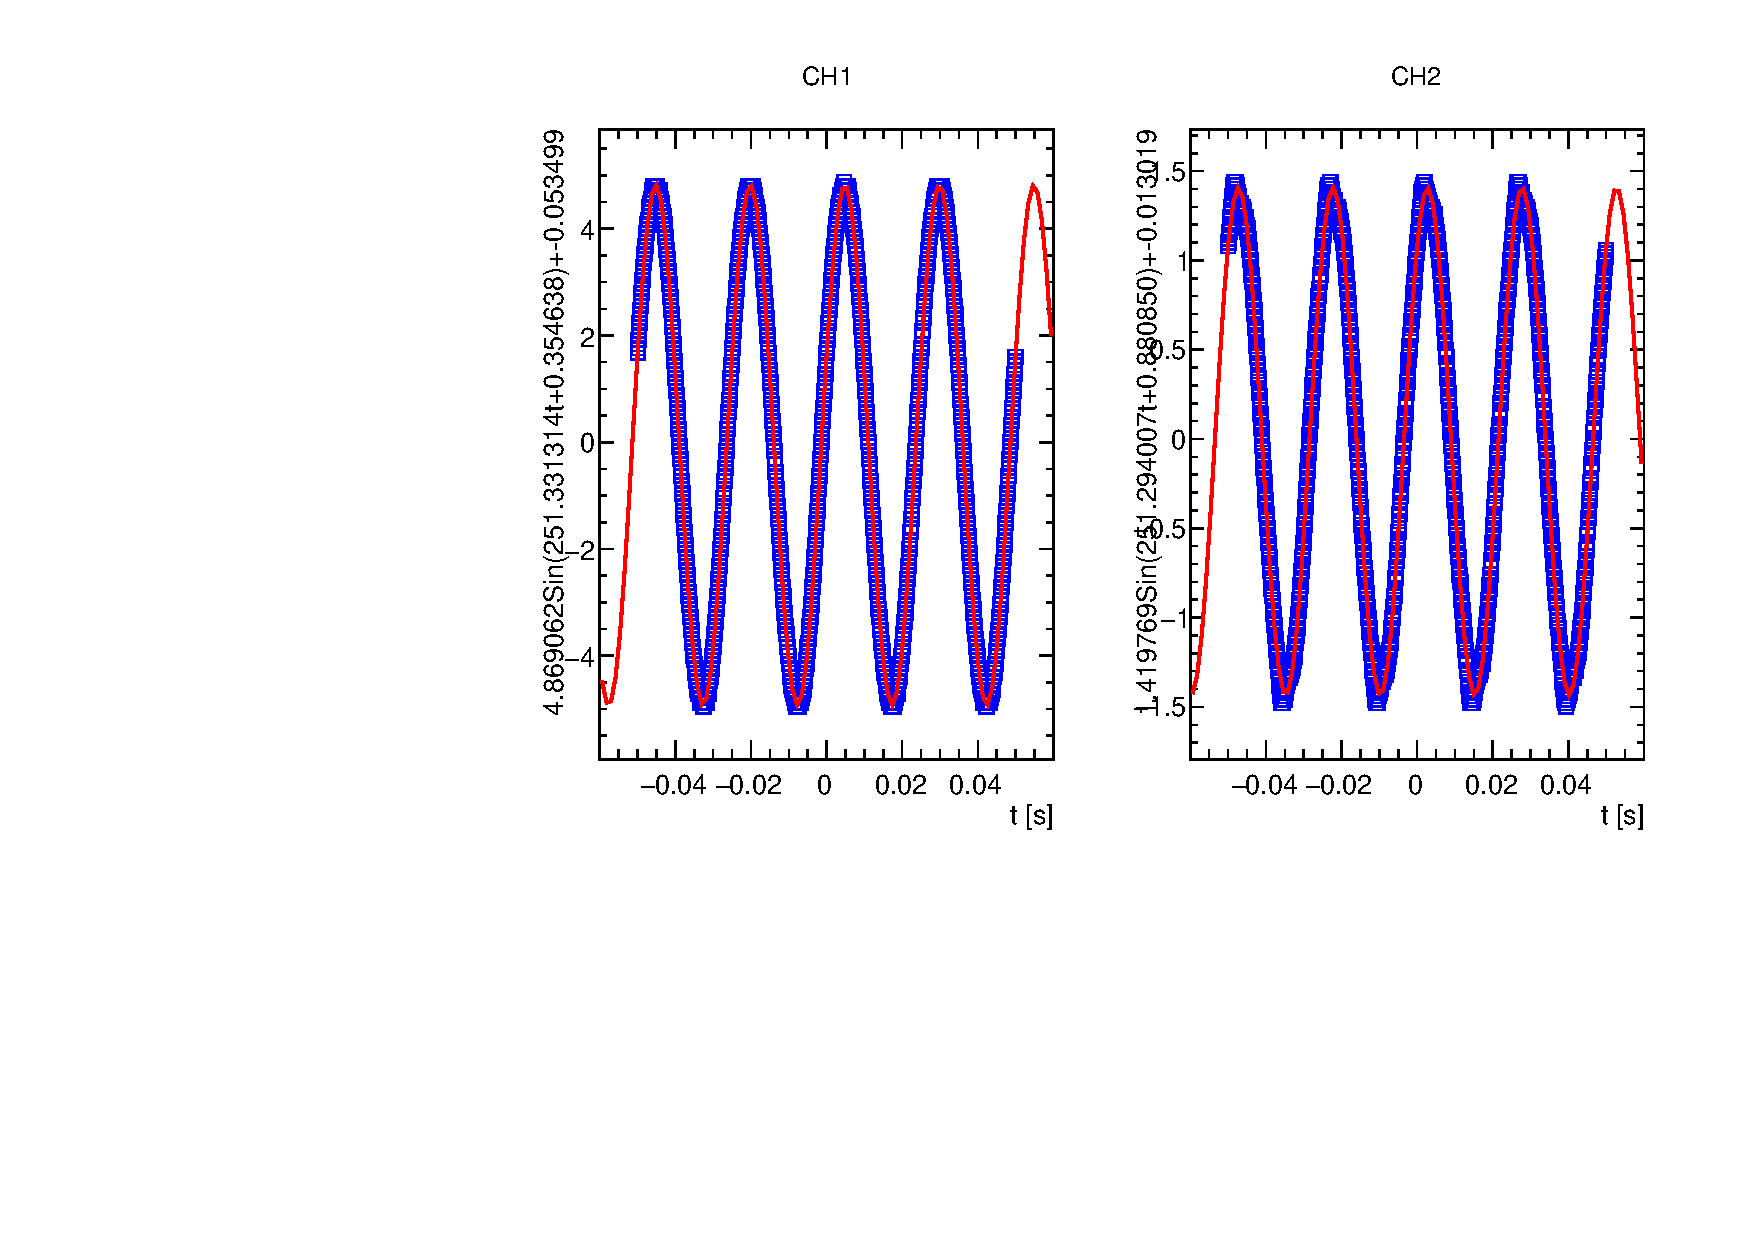
\includegraphics[scale=0.8]{img/fit.pdf}}
\caption{Одна із апроксимованих синусоїд. Біля осей ординат вказані параметри підігнаних синусоїд}
\label{fit}
\end{figure}
\begin{figure}[h]
\center{
    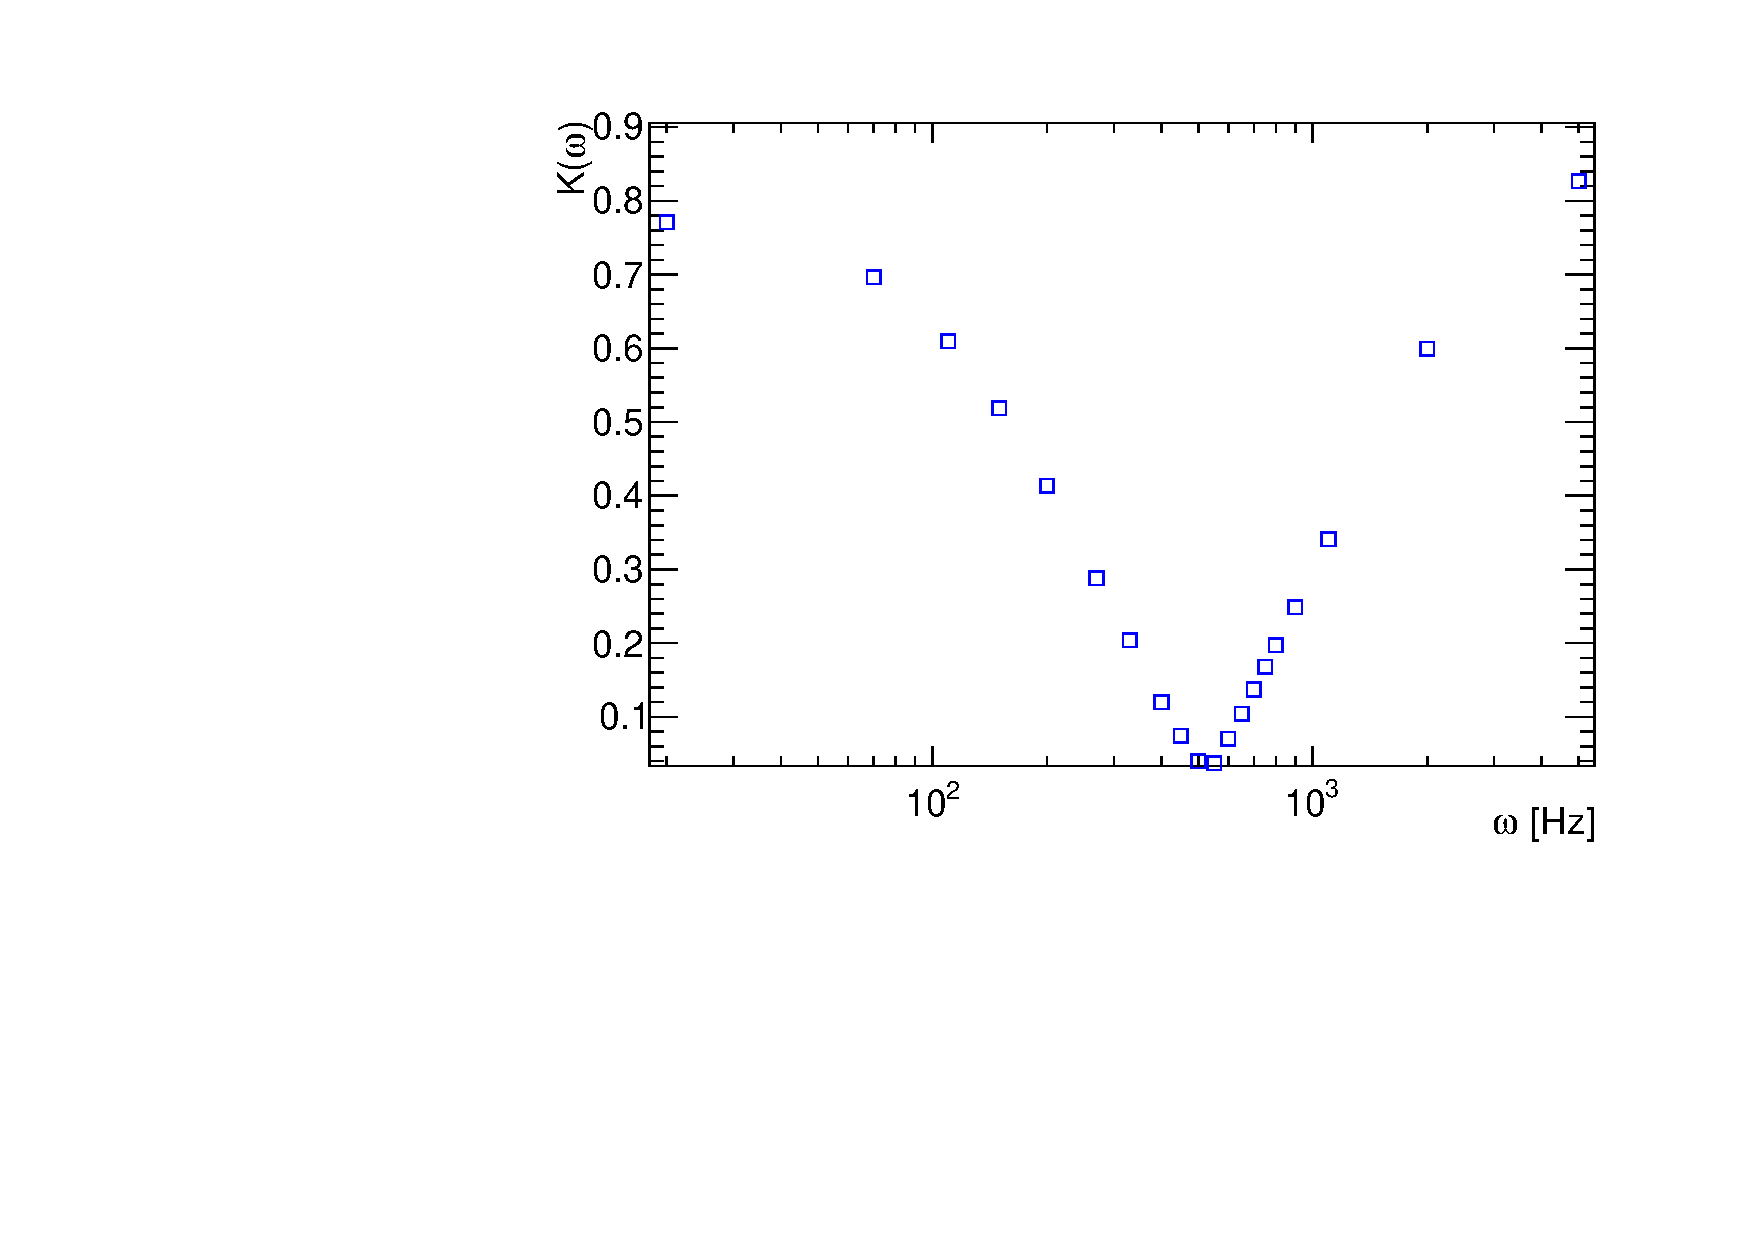
\includegraphics[width=0.45\linewidth]{img/1_K.pdf}
    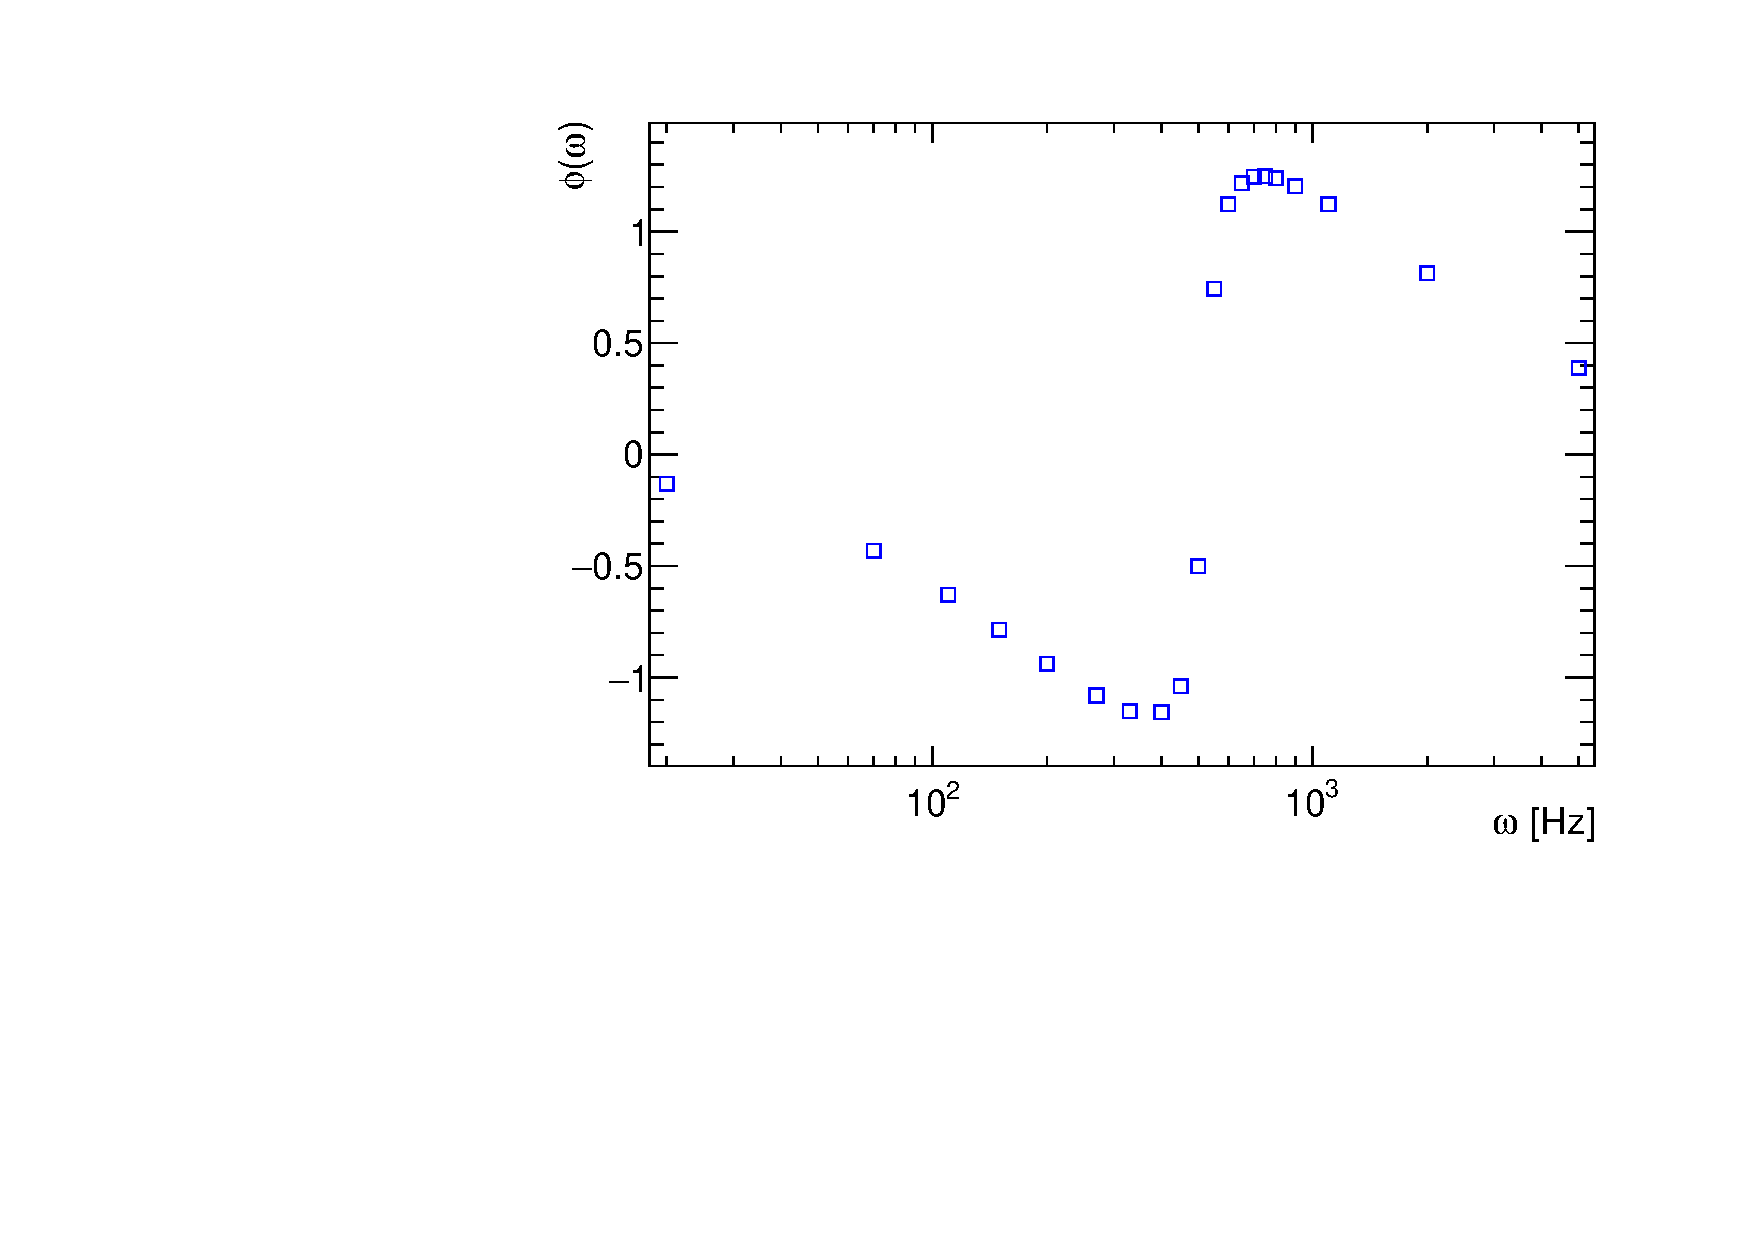
\includegraphics[width=0.45\linewidth]{img/1_Phi.pdf}
}
\caption{АЧХ та ФЧХ для чотирьохполюсника №1. Призначення чотирьохполюсника: "убити" непотрібні частоти.}
\label{res1}
\end{figure}
\begin{figure}[h]
\center{
    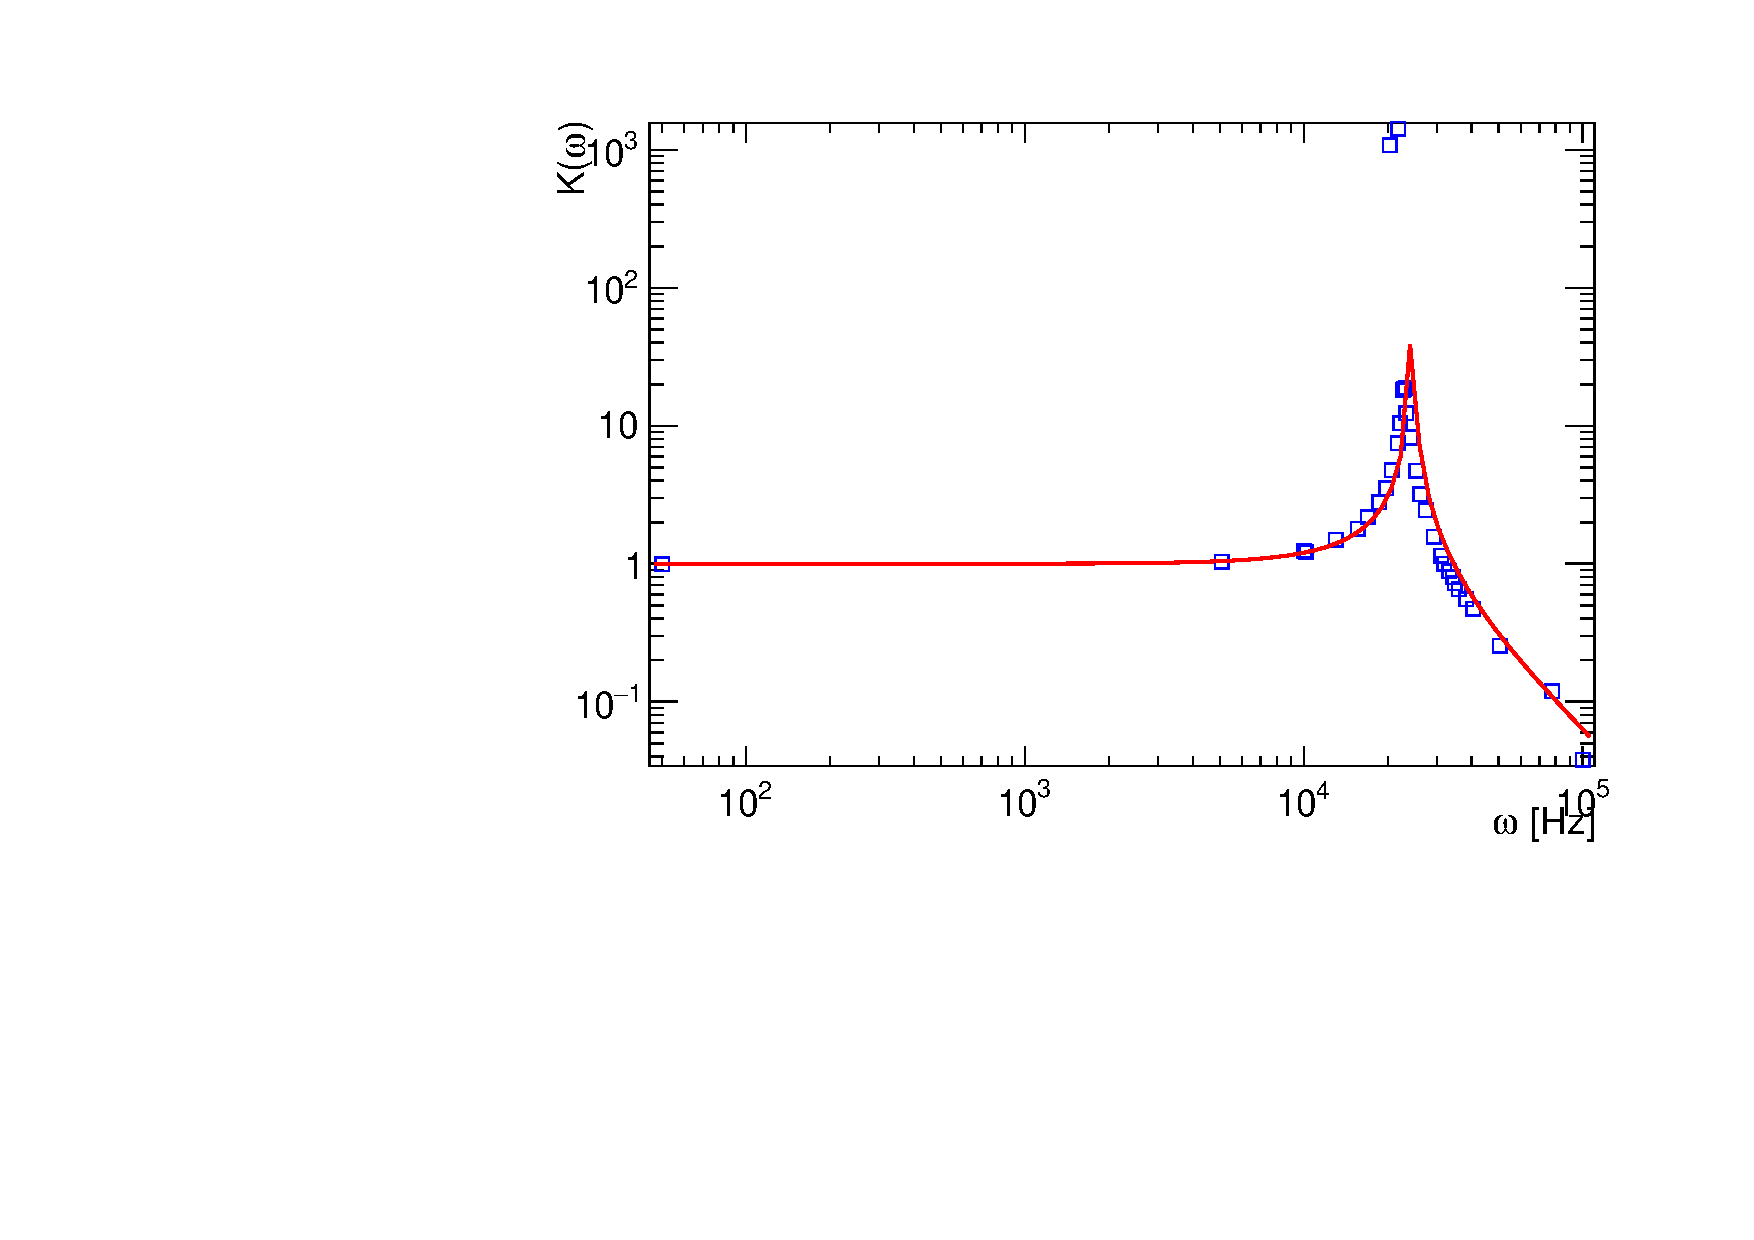
\includegraphics[width=0.45\linewidth]{img/2_K.pdf}
    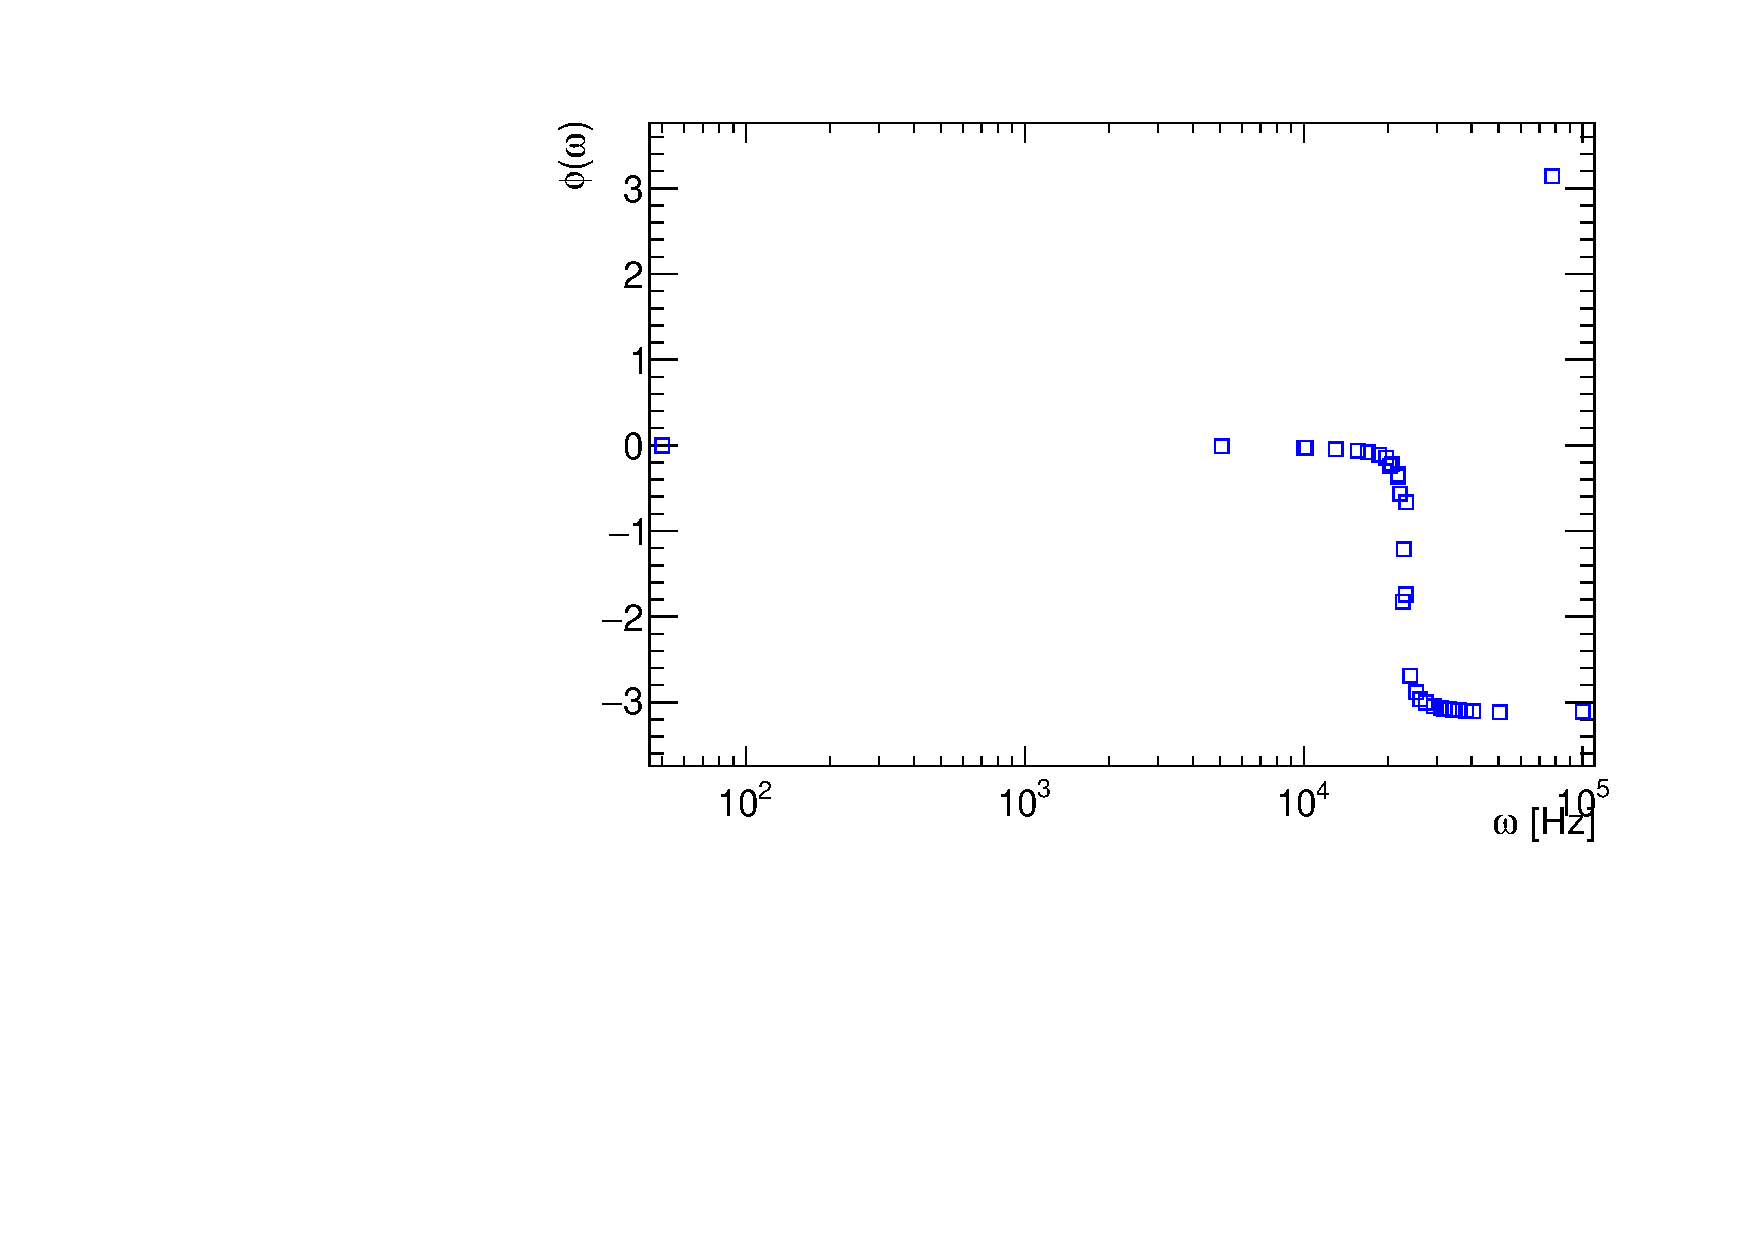
\includegraphics[width=0.45\linewidth]{img/2_Phi.pdf}
}
\caption{АЧХ та ФЧХ для чотирьохполюсника №2. Присутні спроби авторів таки підігнати якусь теоретичну залежність під ці гарні точки. Призначення чотирьохполюсника: підсилити коливання на певній частоті.}
\label{res2}
\end{figure}\begin{figure}[h]
\center{
    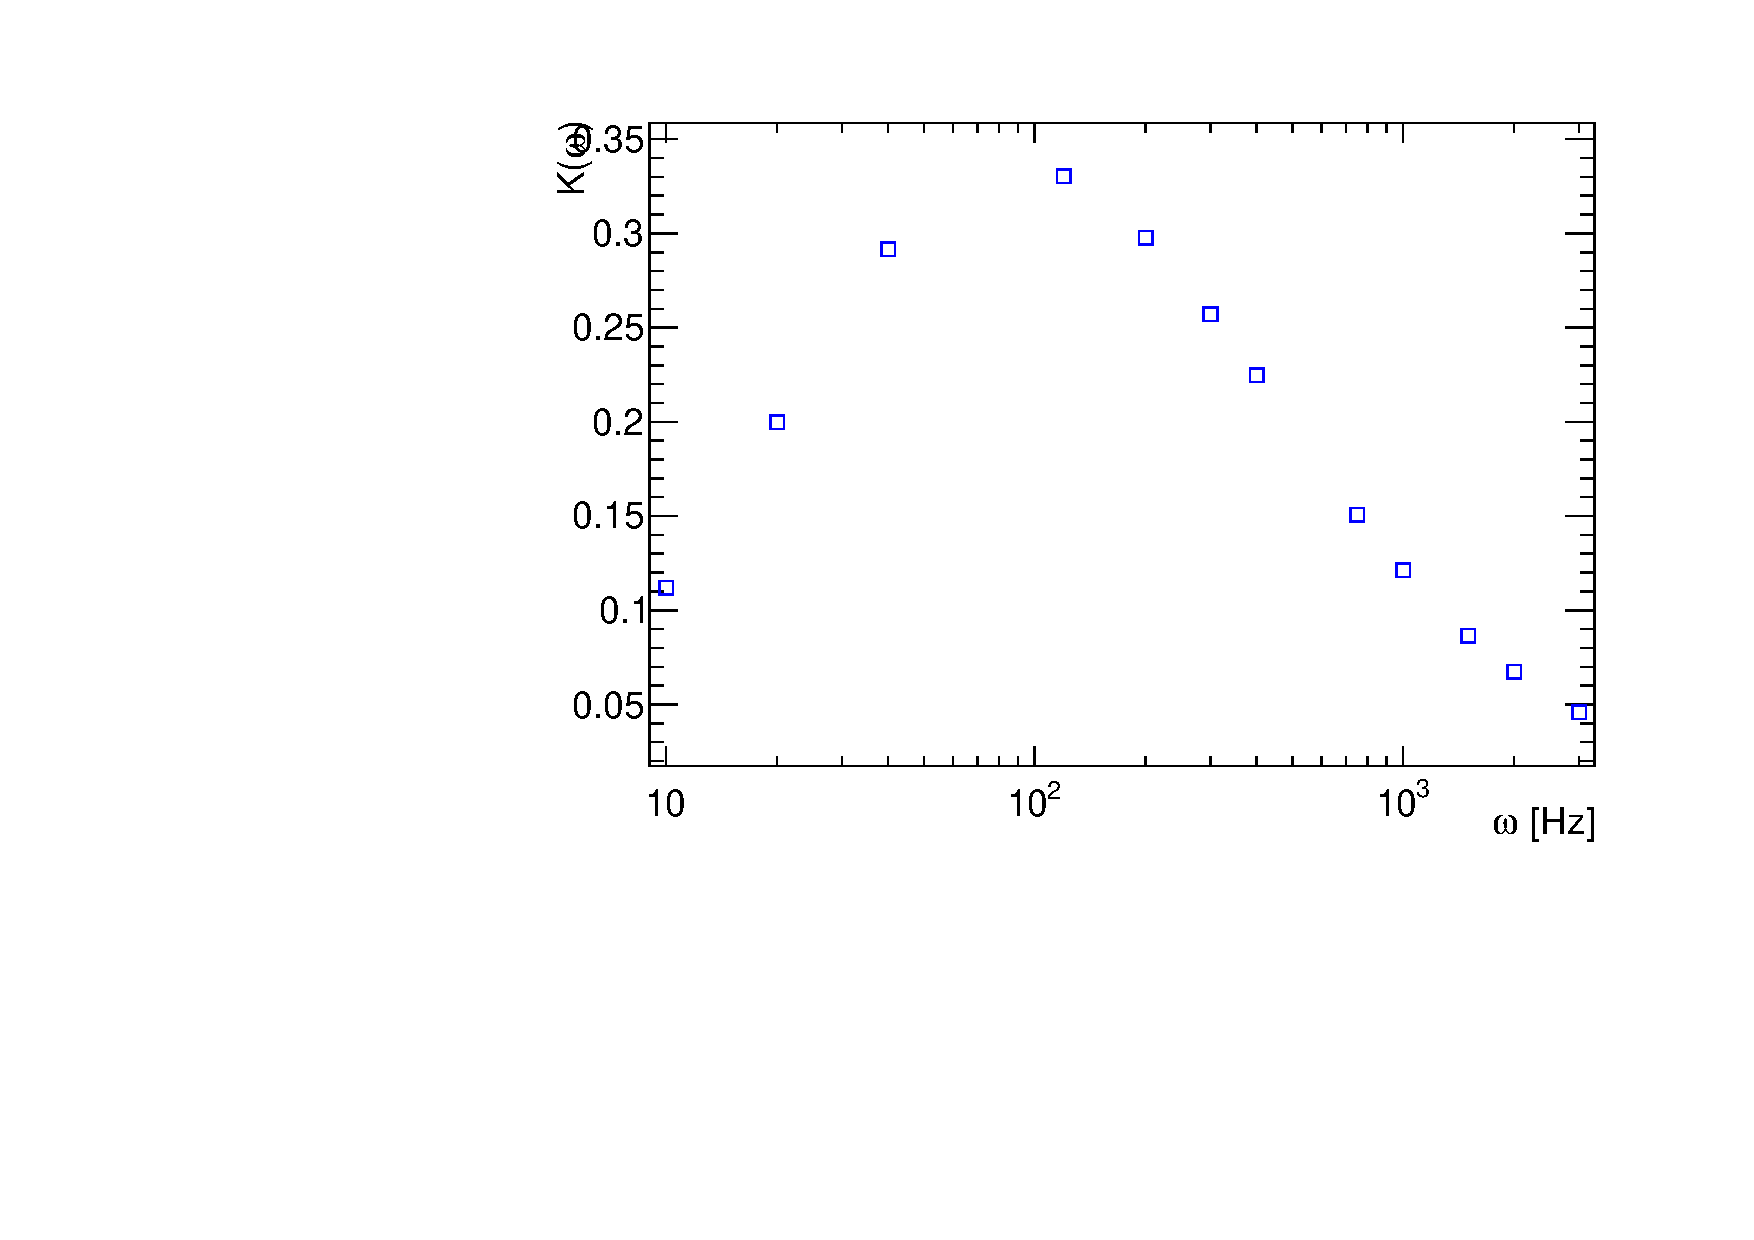
\includegraphics[width=0.45\linewidth]{img/3_K.pdf}
    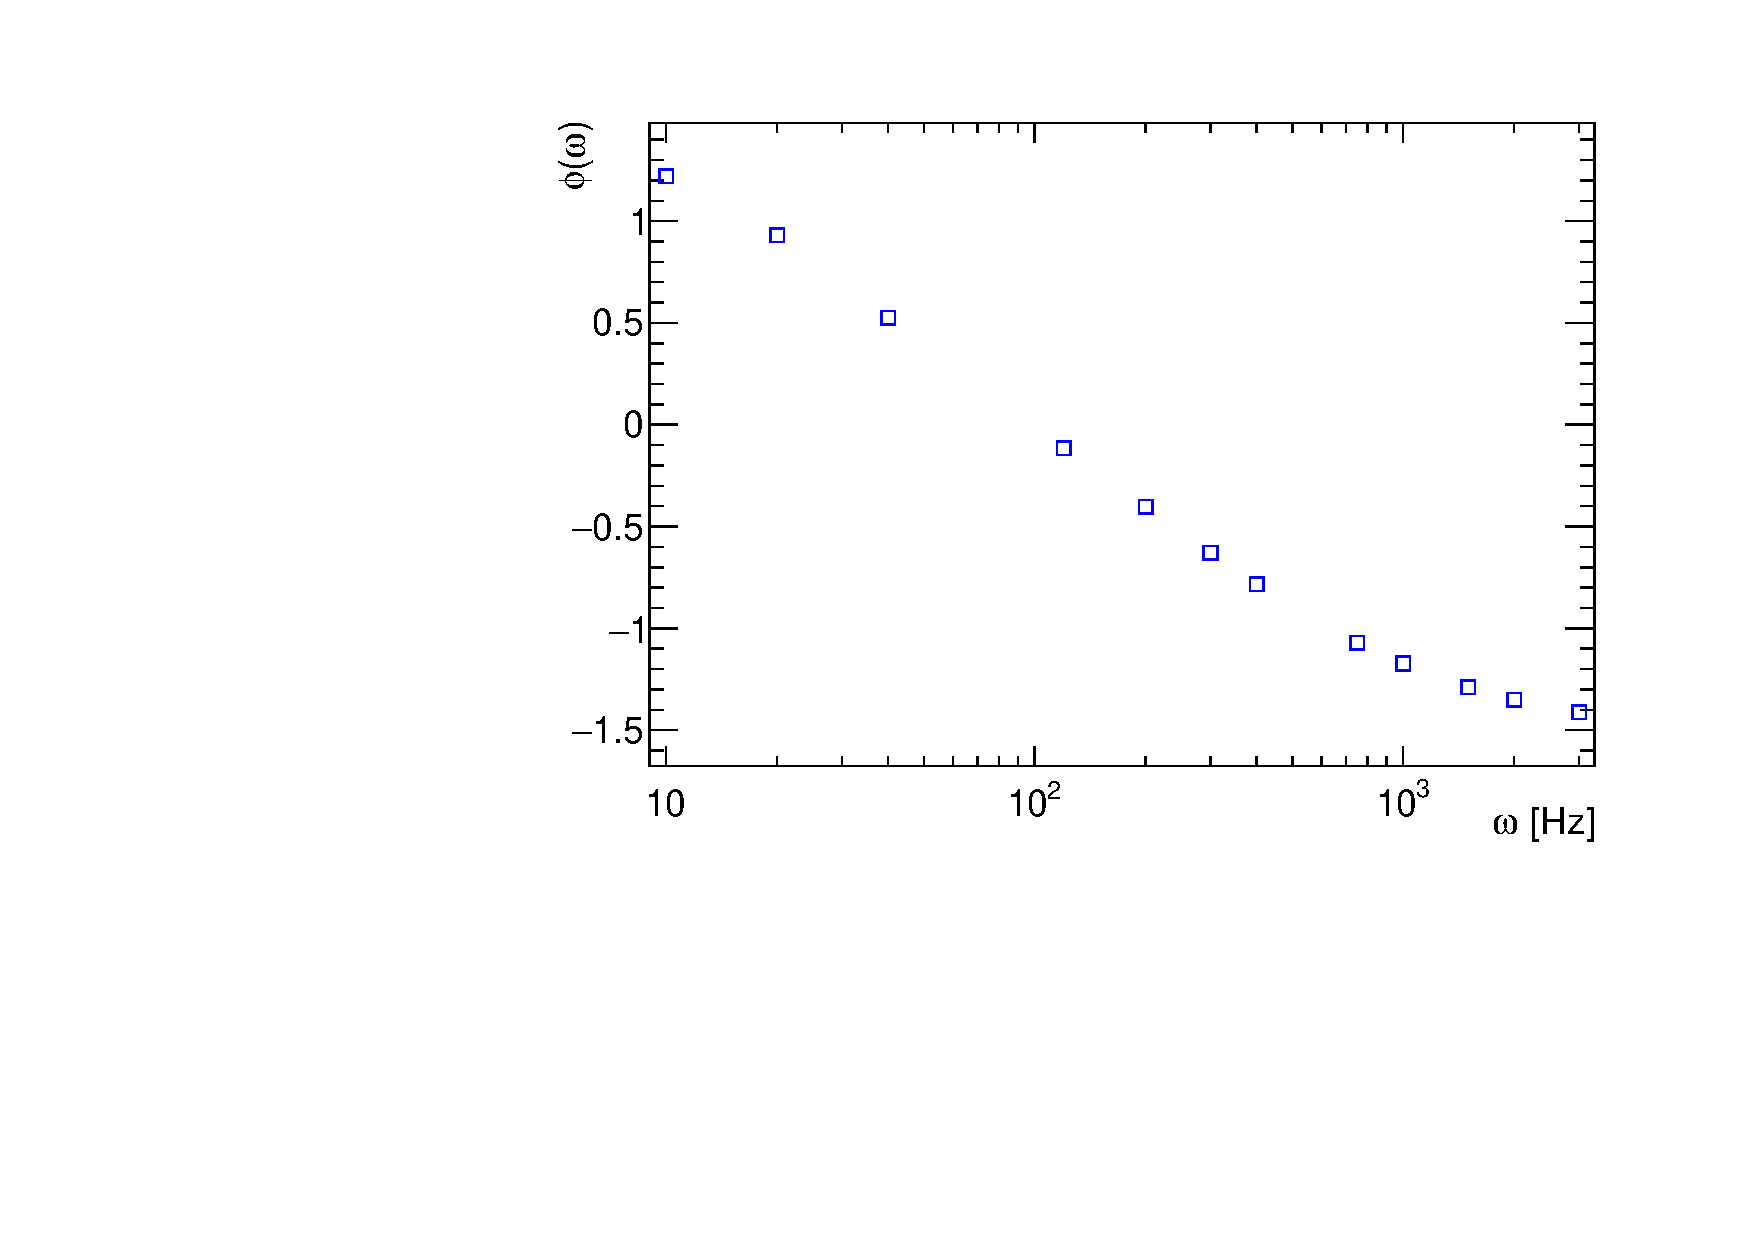
\includegraphics[width=0.45\linewidth]{img/3_Phi.pdf}
}
\caption{АЧХ та ФЧХ для чотирьохполюсника №3. Призначення чотирьохполюсника: подавити всі частоти, але деяким дати шанс на виживання}
\label{res3}
\end{figure}